\section*{Sets}
\addcontentsline{toc}{section}{Sets}

\subsection*{Denoting Sets}
\addcontentsline{toc}{subsection}{Denoting Sets}

A \textbf{set} is simply a collection of objects, or elements.\\
If a set is finite and not large, we can describe it by simply listing the elements:

\begin{center}
\textit{A} = \{1, 2, 3, 4\}
\end{center}


The above set $A$ is made up of four elements.  \textbf{The order of the elements in a set does not matter}, therefore, a could also be specified like so:

\begin{center}
\textit{A} = \{1, 3, 4, 2\}
\end{center}

\textbf{The elements of a set are assumed to be distinct}, so any duplicate occurence of an element can be ignored.  Therefore, we could also specify set $A$ like so:

\begin{center}
\textit{A} = \{1, 2, 2, 3, 4, 4\}
\end{center}


If a set is very large or infinite, we can describe it using a property necessary for membership:

\begin{center}
\textit{B} = $\{x \mid x \text{ is a positive, even integer}\}$
\end{center}

The above set $B$ is made up of positive, even integers.  The vertical bar ``$\mid$'' is read as ``such that'' and the text after the bar is the property.  Therefore, $B$ can be read as ``the set of all x such that x is a positive, even integer.''
Some sets of numbers occur frequently in mathematics and are given symbols.

\begin{table}[]
\begin{tabular}{cll}
\multicolumn{1}{l}{Symbol} & Set              & Example of Members         \\
\textbf{Z}                 & Integers         & -3, 0, 2, 145              \\
\textbf{Q}                 & Rational numbers & -1/3, 0, 24/15             \\
\textbf{R}                 & Real numbers     & -3, -1.766, 0, 4/15, $\sqrt{2}$, 2.666, \dots, $\pi$
\end{tabular}
\end{table}

Rational numbers are quotients of integers, thus \textbf{Q} for \textit{quotient}.  The set of real numbers \textbf{R} consists of all points on a straight line extending indefinitely in either direction.

We can denote the positive elements in a set using the superscript plus (e.g., \textbf{Z\textsuperscript{+}} for positive integers) and the negative elements in a set using the superscript minus (e.g., \textbf{Q\textsuperscript{-}} for negative rational numbers).

\subsection*{Set Cardinality}
\addcontentsline{toc}{subsection}{Set Cardinality}

If \textit{X} is a finite set, we let
\begin{center}
$|X| = \text{number of elements in } X$
\end{center}

We call $|X|$ the \textbf{cardinality} of \textit{X}.\\

If we let \textit{A} = \{1, 2, 3, 4\}, then the cardinality of \textit{A} is 4, or $|A| = 4$.  The cardinality of \{\textbf{R}, \textbf{Z}\} is 2 since it contains two elements, which just happen to be sets.\\\\\textbf{Remember: an element in a set can be anything, even a set.}\\

If \textit{x} is in the set \textit{X}, we write $x \in X$.  If \textit{x} is NOT in the set \textit{X}, we write $x \not\in X$.  For example, both of these are true:

\begin{align*}
    3 &\in \{1, 2, 3, 4\}\\
    3 &\not\in \{x \mid x \text{ is a positive, even integer}\}
\end{align*}

\subsection*{Empty Set}
\addcontentsline{toc}{subsection}{Empty Set}

A set with no elements is called an \textbf{empty set} and is denoted by $\emptyset$.  In other words, $\emptyset = \{\}.$

\clearpage

\subsection*{Set Equality}
\addcontentsline{toc}{subsection}{Set Equality}

Two sets \textit{X} and \textit{Y} are \textbf{equal} ($X = Y$) if \textit{X} and \textit{Y} have the same elements.  To put it differently, for $X = Y$ to be true:

\begin{center}
For every \textit{x}, if $x \in X$, then $x \in Y$\\
For every \textit{x}, if $x \in Y$, then $x \in X$
\end{center}

Here are two examples that demonstrate \textit{equality} among sets:\\

If

\begin{center}
\textit{A} = \{1, 3, 2\} and \textit{B} = \{2, 3, 2, 1\},
\end{center}

then, by inspection, \textit{A} and \textit{B} have the same elements. Therefore $A = B$.\\\\\textbf{Remember: The elements in a set are unique, so duplicates are removed when evaluating a set.}\\

If

\begin{center}
\textit{A} = $\{x \mid x^2 + x - 6 = 0 \}$ and \textit{B} = \{2, -3\},
\end{center}

then, $A = B$ in this case, too.\\

\subsection*{Set Inequality}
\addcontentsline{toc}{subsection}{Set Inequality}

For a set \textit{X} to NOT be equal to a set \textit{Y} ($X \neq Y$), \textit{X} and \textit{Y} must NOT have the same elements.  In other words, there must be at least one element in \textit{X} that is not in \textit{Y} or at least one element in \textit{Y} that is not in \textit{X} (or both).\\

Here is an example that demonstrates \textit{inequality} among sets:\\

If

\begin{center}
\textit{A} = \{1, 3, 2\} and \textit{B} = \{4, 2\},
\end{center}

Then, by inspection, $A \neq B$.
\clearpage

\subsection*{Subsets}
\addcontentsline{toc}{subsection}{Subsets}

Suppose \textit{X} and \textit{Y} are sets.  If every element of \textit{X} is an element of \textit{Y}, we say \textit{X} is a \textbf{subset} of \textit{Y} and write $X \subseteq Y$.  In other words,\\

If

\begin{center}
$X$ and $Y$ are sets and, for every x, $x \in X$ and $x \in Y$.
\end{center}

Then, $X \subseteq Y$.  Here are some examples demonstrating subsets:\\

If

\begin{center}
\textit{C} = \{1, 3\} and \textit{A} = \{1, 2, 3, 4\},
\end{center}

then, every element of \textit{C} is an element of \textit{A}.  Therefore, $C \subseteq A$.\\

Let

\begin{center}
\textit{X} = $\{x \mid x^2 + x - 2 = 0 \}$
\end{center}

We can show that $X \subseteq \textbf{Z}$:\\

Remember, \textbf{Z} is a set of integers, so

\begin{center}
    \textbf{Z} = $\{x \mid x \text{ is an integer}\}$.
\end{center}

We can solve for the subset \textit{X}

\begin{align*}
x^2 + x - 2 &= 0\\
(x+2)(x-1) &= 0
\end{align*}

which gives $x = -2 \text{ and } x = 1$. So \textit{X} = \{-2, 1\}.  Since every element of set \textit{X} is an element of set \textbf{Z}, $X \subseteq \textbf{Z}$.

\clearpage

For a set \textit{X} to NOT be a subset of a set \textit{Y}, there must be at least one element of \textit{X} that is NOT a member of \textit{Y}.\\

Let

\begin{center}
\textit{X} = $\{x \mid 3x^2 - x - 2 = 0 \}$
\end{center}

We can show that \textit{X} is NOT a subset of \textbf{Z}:\\

If $x \in X$, then

\[
    3x^2 - x - 2 = 0.
\]

Solving for \textit{x}, we obtain $x = 1 \text{ and } x = -\frac{2}{3}$, so $X = \{1, -\frac{2}{3}\}$.  Since $-\frac{2}{3} \not\in \textbf{Z}$, \textit{X} is NOT a subset of \textbf{Z}.\\

Given a set \textit{X}, $X \subseteq X$, since every element of \textit{X} is an element of itself.\\

\subsection*{Proper Subsets}
\addcontentsline{toc}{subsection}{Proper Subsets}

If \textit{X} is a subset of \textit{Y} and $X \neq Y$, then \textit{X} is a \textbf{proper subset} of $Y$ and we write $X \subset Y$.  If $X \subset Y$, then $X$ is ALWAYS smaller than $Y$.\\

Let

\begin{center}
\textit{C} = \{1, 3\} and \textit{A} = \{1, 2, 3, 4\},
\end{center}

Then $C \subset A$ since $C \neq A$.\\


\textbf{Understanding subsets versus proper subsets:}

\begin{itemize}
\item The symbol for a subset ($\subseteq$) is analogous to $\leq$.  In other words, a subset \textit{can} be the same size as the parent set.
\item The symbol for a proper subset ($\subset$) is analogous to $<$.  In other words, a proper subset is smaller than the parent set.
\end{itemize}

\clearpage

\subsection*{Power Set}
\addcontentsline{toc}{subsection}{Power Set}

The set of all subsets (proper or not) of a set $X$, denoted $\mathcal{P}(X)$, is called the \textbf{power set} of 
$X$.\\

If $A$ = \{a, b, c\}, then

\begin{center}
$\mathcal{P}(A) = \{\emptyset, \{a\}, \{b\}, \{c\}, \{a, b\}, \{a, c\}, \{b, c\}, \{a, b, c\}\}$.
\end{center}

All but \{a, b, c\} are proper subsets of $A$. $|A| = 3$ and $|\mathcal{P}(A)| = 2^3 = 8$.\\\\
In other words, given a set $X$ with $n$ elements, $|\mathcal{P}(X)| = 2^n$. 

Given two sets $X$ and $Y$, there are several operations that can be performed on the sets to produce a new set.\\

\subsection*{Union, Intersection, and Difference}
\addcontentsline{toc}{subsection}{Union, Intersection, and Difference}

The \textbf{union} of $X$ and $Y$,

\[
    X \union Y = \{x \mid x \in X \text{ or } x \in Y\},
\]

is a set that consists of all elements belonging to $X$ or $Y$ (or both).\\

The \textbf{intersection} of $X$ and $Y$,

\[
    X \intersection Y = \{x \mid x \in X \text{ and } x \in Y\},
\]

is a set that consists of all elements belonging to $X$ and $Y$.\\

The \textbf{difference} of $X$ and $Y$,

\[
    X - Y = \{x \mid x \in X \text{ and } x \not\in Y\},
\]

is a set that consists of all elements in $X$ that are not in $Y$.\\

If

\begin{center}
A = \{1, 3, 5\} and B = \{4, 5, 6\}
\end{center}

then, 

\begin{align*}
    A \union B &= \{1, 3, 4, 5, 6\}\\
    A \intersection B &= \{5\}\\
    A - B &= \{1, 3\}\\
    B - A &= \{4, 6\}
\end{align*}

\textbf{In general, A - B $\neq$ B - A.}\\

\subsection*{Union of a Family of Sets}
\addcontentsline{toc}{subsection}{Union of a Family of Sets}

Just like how we took the union of two sets above, we can take the union of a family of sets $\mathcal{S}$.\\

We define the union of a family $\mathcal{S}$ of sets to be those elements $x$ belonging to at least one set $X$ in the family $\mathcal{S}$.  In other words,

\begin{center}
    $\union$ $\mathcal{S} = \{x \mid x \in X \text{ for some } X \in \mathcal{S}\}$.
\end{center}

We can calculate the union of $\mathcal{S}$ like so:

\begin{center}
    $\bigcup$ $\mathcal{S} = \bigcup\limits_{i=1}^{n} X_i$
\end{center}
\begin{center}
where $X$ is some set in $\mathcal{S}$ and $n$ is the cardinality of $\mathcal{S}$.
\end{center}

Let

\begin{align*}
    A_1 &= \{1, 2, 6, 7, 9\}\\
    A_2 &= \{2, 5, 6, 7, 8, 9, 10\}\\
    A_3 &= \{1, 2, 3, 4, 9\}\\
    \mathcal{S} &= \{A_1, A_2, A_3\}
\end{align*}

Then, the union of $\mathcal{S}$ is 

\begin{center}
    $\bigcup$ $\mathcal{S} = \bigcup\limits_{i=1}^{3} A_i = A_1 \union A_2 \union A_3 = \{1, 2, 3, \dots, 10\}$. 
\end{center}

\subsection*{Intersection of a Family of Sets}
\addcontentsline{toc}{subsection}{Intersection of a Family of Sets}

Just like how we took the intersection of two sets above, we can take the intersection of a family of sets $\mathcal{S}$.\\

We define the intersection of a family $\mathcal{S}$ of sets to be those elements $x$ belonging to at least one set $X$ in the family $\mathcal{S}$.  In other words,

\begin{center}
    $\intersection$ $\mathcal{S} = \{x \mid x \in X \text{ for all } X \in \mathcal{S}\}$.
\end{center}

We can calculate the intersection of $\mathcal{S}$ like so:

\begin{center}
    $\bigcap$ $\mathcal{S} = \bigcap\limits_{i=1}^{n} X_i$
\end{center}
\begin{center}
where $X$ is some set in $\mathcal{S}$ and $n$ is the cardinality of $\mathcal{S}$.
\end{center}

Let

\begin{align*}
    A_1 &= \{1, 2, 6, 7, 9\}\\
    A_2 &= \{2, 5, 6, 7, 8, 9, 10\}\\
    A_3 &= \{1, 2, 3, 4, 9\}\\
    \mathcal{S} &= \{A_1, A_2, A_3\}
\end{align*}

Then, the intersection of $\mathcal{S}$ is 

\begin{center}
    $\bigcap$ $\mathcal{S} = \bigcap\limits_{i=1}^{3} A_i = A_1 \intersection A_2 \intersection A_3 = \{2, 9\}$. 
\end{center}

\subsection*{Disjoint Sets}
\addcontentsline{toc}{subsection}{Disjoint Sets}

Sets $X$ and $Y$ are \textbf{disjoint} if $X \intersection Y = \emptyset$.  In other words, if $X$ and $Y$ share no elements, they are disjoint.

\subsection*{Pairwise Disjoint}
\addcontentsline{toc}{subsection}{Pairwise Disjoint}

A collection of sets $\mathcal{S}$ is said to be \textbf{pairwise disjoint} if every pair of sets within the set are disjoint.\\

Let

\begin{center}
    $\mathcal{S}$ = \{$A_1$, $A_2$, $A_3$, \dots, $A_n$\}.
\end{center}

If

\begin{center}
    For every $i$ and $j$ in $\mathcal{S}$, $A_i \intersection A_j = \emptyset$, where $i \neq j$.
\end{center}

then, $\mathcal{S}$ is a pairwise disjoint set.\\

For example, If

\begin{center}
    $\mathcal{S}$ = \{\{1, 4, 5\}, \{2, 6\}, \{3\}, \{7, 8\}\}.
\end{center}

then, by inspection, $\mathcal{S}$ is pairwise disjoint because no set within $\mathcal{S}$ contains common elements.

\subsection*{Universal Set}
\addcontentsline{toc}{subsection}{Universal Set}

Every set is a subset of $U$, which is the universal set.  The universal set must be explicitly defined or given from context.

\subsection*{Complement Set}
\addcontentsline{toc}{subsection}{Complement Set}

A set $\overline{X} = U - X$ is the \textbf{complement} of $X$.  In other words, a \textit{complement} of a set $X$ is the set that contains all elements except those in $X$.\\

Let
\begin{align*}
    A &= \{1, 3, 5\}\\
    U &= \{1, 2, 3, 4, 5\}.
\end{align*}

Then the complement of $A$ is

\begin{center}
    $\overline{A} = U - A = \{2, 4\}$
\end{center}

\subsection*{Venn Diagrams}
\addcontentsline{toc}{subsection}{Venn Diagrams}

\textbf{Venn Diagrams} provide pictorial views of a set.  In a Venn Diagram, a rectangle depicts a universal set.  Subsets of the universal set are drawn as circles, and the members of a set are within the circle.

\begin{figure}[h]
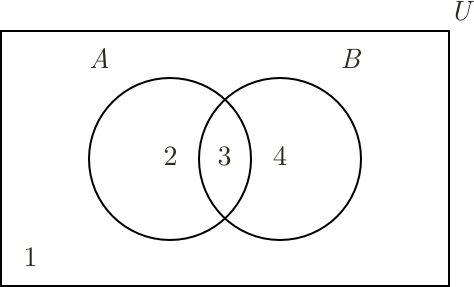
\includegraphics[width=8cm]{./01/01/venn-diagram}
\centering
\end{figure}

In the above diagram,

\begin{align*}
    1 &= \overline{(A \union B)}\\
    2 &= A - B\\
    3 &= A \intersection B\\
    4 &= B - A\\
\end{align*}

\clearpage

\subsection*{Ordered Pairs}
\addcontentsline{toc}{subsection}{Ordered Pairs}

As previously stated, a set is an \textit{unordered} collection of elements.  However, sometimes we want to consider the order of elements.  An \textbf{ordered pair} of elements, written $(a, b)$, is considered distinct from $(b, a)$ so long as $a \neq b$.  

\subsection*{Cartesian Product}
\addcontentsline{toc}{subsection}{Cartesian Product}

If $X$ and $Y$ are sets, we let $X \times Y$ denote the set of all ordered pairs $(x, y)$, where $x \in X, y \in Y$.  We call this set of ordered pairs a \textbf{Cartesian product}.\\

If $X = \{1, 2, 3\}$ and $Y = \{a, b\}$, then
\begin{align*}
X \times Y &= \{(1, a), (1, b), (2, a), (2, b), (3, a), (3, b)\}\\
Y \times X &= \{(a, 1), (b, 1), (a, 2), (b, 2), (a, 3), (b, 3)\}
\end{align*}

Note, in general, $X \times Y \neq Y \times X$.  Also note that $|X \times Y| = |X| \cdot |Y| = 6$.\\
It is always true that $|X \times Y| = |X| \cdot |Y|$.\\

If $X = \{1, 2\}$ and $Y = \{a, b\}$, and $Z = \{\alpha, \beta\}$, then
\begin{align*}
    X \times Y \times Z = \{(1, a, \alpha), (1, a, \beta), (1, b, \alpha), (1, b, \beta), (2, a, \alpha), (2, a, \beta), (2, b, \alpha), (2, b, \beta)\}
\end{align*}

\subsection*{Set Laws}
\addcontentsline{toc}{subsection}{Set Laws}

Let $U$ be a universal set and sets $A$, $B$, and $C$ be subsets of $U$.  The following properties hold.\\

\textbf{Associative laws:}
\begin{align*}
    (A \union B) \union C &= A \union (B \union C)\\
    (A \intersection B) \intersection C &= A \intersection (B \intersection C)
\end{align*}

\textbf{Commutative laws:}
\begin{align*}
    A \union B &= B \union A\\
    A \intersection B &= B \intersection A
\end{align*}

\clearpage

\textbf{Distributive laws:}
\begin{align*}
    A \intersection (B \union C) &= (A \intersection B) \union (A \intersection C)\\
    A \union (B \intersection C) &= (A \union B) \union (A \union C)
\end{align*}

\textbf{Identity laws:}
\begin{align*}
    A \union \emptyset = A, A \intersection U = A
\end{align*}

\textbf{Complement laws:}
\begin{align*}
    A \union \overline{A} = U, A \intersection \overline{A} = \emptyset
\end{align*}

\textbf{Idempotent laws:}
\begin{align*}
    A \union A = A, A \intersection A = A
\end{align*}

\textbf{Bound laws:}
\begin{align*}
    A \union U = U, A \intersection \emptyset = \emptyset
\end{align*}

\textbf{Absorption laws:}
\begin{align*}
    A \union (A \intersection B) = A, A \intersection (A \union B) = A
\end{align*}

\textbf{Involution law:}
\begin{align*}
    \overline{\overline{A}} = A
\end{align*}

\textbf{0/1 laws:}
\begin{align*}
    \overline{\emptyset} &= U\\
    \overline{U} &= \emptyset
\end{align*}

\textbf{De Morgan's laws for sets}
\begin{align*}
    \overline{(A \union B)} &= \overline{A} \intersection \overline{B}\\
    \overline{(A \intersection B)} &= \overline{A} \union \overline{B}
\end{align*}








